\documentclass[a4paper, 11pt]{article}

\usepackage{geometry}
\geometry{a4paper,left=30mm,right=30mm, top=35mm, bottom=30mm}

\usepackage[english]{babel}
\usepackage[utf8]{inputenc} 
\usepackage[T1]{fontenc}
\usepackage{amsmath}
\usepackage{amssymb}
\usepackage{fancyhdr}
\usepackage{graphicx}
\usepackage{hyperref}
\usepackage{csquotes}

\usepackage{lastpage} % Seitenzahlen

\pagestyle{fancy}
\usepackage{amsmath}
\usepackage{tabularx} %schöne tabellen
\parindent0pt %einrücken verhindern
\renewcommand{\familydefault}{\sfdefault} % use sans fonts


\cfoot{\thepage  \ / \pageref{LastPage}}

\usepackage[
backend=biber,
style=alphabetic,
citestyle=authoryear
]{biblatex}

\graphicspath{{./images/}}

\DeclareMathOperator*{\argmin}{argmin} % no space, limits underneath in displays

% % % % % % % % % % % % % % % % % % % % % % % %
% % % % % % % % % % % % % % % % % % % % % % % %
\newcommand{\thesis}{Bachelor Thesis}
\newcommand{\topic}{Using Approximate Bayesian Computation to Infer the Number of Populations from SNP Genotype Data}
\newcommand{\modul}{Bachelor Thesis}
\newcommand{\supervisor}{Supervisors: Manfred Opper, \\ Olivier Fran\c{c}ios, \\ Michael Blum}
 \newcommand{\name}{Fabian Bergmann}
\newcommand{\datum}{\today}
% % % % % % % % % % % % % % % % % % % % % % % %
% % % % % % % % % % % % % % % % % % % % % % % %


\addbibresource{sources.bib}

\begin{document} 

%%% Kopfzeile linker Bereich
%      gerade Seite   ungerade Seite
\lhead[ \leftmark   ]{\textbf{\modul}}
%%% Kopfzeile mittlerer Bereich
%      gerade Seite   ungerade Seite
\chead[\rightmark   ]{\rightmark{}}
%%% Kopfzeile linker Bereich
%      gerade Seite             ungerade Seite
\rhead[\textbf{text}]{\name}


	%-- Deckblatt --						      
  \title{\textbf{\thesis\\[0.5cm] \Large{\topic} \\[1.5cm]}
	\author{%\tutorium\\ \\
		Fabian Bergmann, 372918\\ \\ \\ \\ \\ \\ \\ \\ 
		Pages: \pageref{LastPage} \\ \\ \\ \\
		}
	\normalsize{\supervisor}} %Thema ändern	
	\date{Submission Date: \datum} %Datum ändern
	\maketitle
	\newpage
	
%\renewcommand{\labelenumi}{\alph{enumi})}
\renewcommand{\labelenumii}{(\roman{enumii})}
%\renewcommand{\labelenumiii}{\arabic{enumiii}.}
%\renewcommand{\labelenumii}{\textbf{-}}	
%-- Eigentlicher Text --

\tableofcontents

\newpage

\section{Introduction}
A central objective in population genetics is to eveluate population structure. Genetical differences of member individuals are analysed  to detect systematic genetic similarities and dissamilarites that could indicate the presence of various subpopulations. The biological definition of a population generally follows the lines of: a population is a "group of organisms of the same species living within a sufficiently restricted geographical area so that any member can potentially mate with any other member of the oppisite sex". Subsequently however, as only a theoretical setting is assumed without any further context, like geography, social hierarchy etc., a population will describe a group of individuals that are associated with one another because their genetic information is  sufficiently homogenous to be discriminated as a group from other individuals of the species. An adpted notion of a subpopulation will not be necessary since the described understanding of a population overlaps with that of a subpopulation (each detectable subpopulation would be a new population), also no further hierarchical structure is present in the used theoretical framework that would make further granulation necessary.\\
An allele is a variant of a gene found at a specific location on a chromosome (locus), and consequently alleles are responsible for the appearance of genetic variation in a species. An allele frequency describes the probability $p(a | k)$ that an individual from population $k$ has the allele $a$. Since individuals in a population possess similar genotypes, so some alleles are encountered more frequently in these individuals than others and what therefore sets them apart, the allele frequencies sufficiently summarise the population.\\
The ampleness of information usually found in a genom poses a challenge dimensionality wise if all of it were to be captured. For tasks that solely involve the analysis of genetic variation between individuals and groups of individuals it suffices to rely on the evaluation of a limited amount of genes. Mostly genese are chosen that are known to be subject to genetic variation, these particular genes are called markers. \textbf{introduce snp markers now?} \\
The usual approach to investigate population structure follows the construction of a statistical model according to biological hypotheses which is then evaluated with respect to how well it fits collected genotype data. The goodness of fit could be evaluated by some statistical means such as hypothesis testing, or by comparison with other models that are based on different biological hypotheses.  Many models thereby employ hyperparameters that demand the specifiaction of their values. The hyperparameter values have to be chosen carefully, since for example by merely picking the parameter values that maximise the likelihood of the model could lead to unrealistic values (especially if model assumptions are faulty). In addition, the comparison of models becomes at best tricky if they both propose different values for the same hyperparameters. A tool that estimates realistic hyperparameter values model independent would therfore be of great facilitation to the inference and evaluation process.\\
One particular hyperparameter that is frequently required in population genetics is the specifiaction of how many populations are present in the to be analysed data, however until now no automated solution exists that satisfyingly and reliably predicts a realistic value. Throughout the following pages an approximate bayesian computation method is presented that intends to deliver a reasonable and fairly neutral estimate for the number of populations in given genotype data.\\
It is fundamentally based on the insight that the behaviour of the spectrum of a covariance matrix is closely linked to the clustering structure found in the respective data. In summary, for $k$ distinguishable (linearly independnt) clusters $k-1$ eigenvalues can be observed that are significantly larger than the rest. This knowledge is consequently exploited to construct a summary statistics, necessary for a lower dimensional computation, solely based on the eigenvalues of the data covariance matrix.\\
In the past methods have been attempted that rely on the same insight, however these mostly use heuristic approaches that intend to identify the jump transition from the lowest large significant eigenvalue to the smaller ones. The results are at best mixed, particularly for data that is noisy and where data structure is not easily detectable. In contrast, the subsequently proposed method attempts to generalise the connection between eigenvalues of the covariance matrix and number of populations by employing a supervised learning approach with boosted decision trees.\\
As for any supervised learning method, a sufficient amount of labeled data will be required to train the model. Constructing an extensive training data set with real genotype data is highly intricate and resource demanding, furthermore, even if an ample amount of consistent genotype data were available, labeling it with the ground truth would be impossible. Of course no method exists that would deliver an unambigous estimate for the number of populations, mostly for the reason that for many real world data sets no unambigous answer can be made. Real genotype data often exhibits a more complex structure. Populations as already indicated are subject to a hierarchical population structure, such that the number of populations detected will depend on the assumptions about what is a population.\\
The biological definition of a population generally follows the lines of: a population is a "group of organisms of the same species living within a sufficiently restricted geographical area so that any member can potentially mate with any other member of the oppisite sex". However, transfering this definition into a theoretical setting without any further real world context, like geography, social hierarchy, etc., is cumbersome if not even impossible for the porpuses of generalistion. Therefore, subsequently a population will describe a substantially large enough group of individuals from the same species that are associated with one another because their genetic information is sufficiently homogenous for them to be discriminated as a whole from other specie individuals. \\
As elicited, the inference of the number of populations is always succumbed by some assumption about the nature of a population. Nevertheless the model assumptions, learned in a supervised learning  approach through the training data, is kept as universal and neutral as possible. The training data, which is supposed to resemble real SNP genotype data samples, is synthetically generated by a generative model, which can simulate a variety of population structure scenarios based on well accepted biological assumptions. Apart from that, the training data is generated as assumptionless as possible.\\
At the core of the generative model lies the idea that a new population splits of from an existing population if for a substantial amount of time a group of individuals of the existing population only interbreed with one another. In a real world context a reason for the split off could for example be that the group decides to settle at different geographic location and thus isolates itself. The general observed genotype of a population is always changed by a force called random genetic drift. If two groups of individuals from the same species do not exchange genetic information by mating, both groups exhibit a different genetic drift such that their genotypes become dissimilar enough to classify them as two seperate populations. \textbf{Furthermore, the use of summary statistics decreases model dependency and improves generality???}

assumptions that are learned by the supervised learning model are kept as universal and neutral as possible to guarentee the transferbility of its predictions.
\textbf{add to discussion, what definition of a population did the model gather}
In this sense an assumption free inference of the number of populations is anyways impossible.

Fundamental to the method is the insight that 
Thereby Usually for this purpose the validity of a certain model is evaluated by analysing the underlying genotype data of the organisms. Models are often susceptible to the realistic choice of hyperparameters, such that for example the likelihood of a model with a certain hyper parameter greater is than for a much more realistc hyper parameter. Since for many models the declaration of the number of populations in the given data is crucial to infer the remaining parameters, a successful and stable technique for determining this parameter would lead to a significant facilitation for the inference process.  \\
  The eigenvalues are therefore a fruitful choice as summary statistics, in order to decrease the dimensionality in the calculation. The likelihood function for this problem is elusive, therefore a gradient boosting tequnique with decision trees wil be employed to bypass its explicit computation. \\
Gradient Boosting is a supervised machine learning method, thus it requires a significant amount of data for training and testing. Real world genotype data however is too extensiv to acquire in such a magnitude as is necessary, therefore an artificial data set is simulated and used. The generation of the artificial data follows commonly accepted theories for the simulation of population structure.

\subsection{Problem}
An allele is a variant of a gene found at a specific location on a chromosome (locus). Its existence originates from a random mutation in a gene. Alleles found at the same locus are generally considered to be interchangeable which allows for the random passing on of an allele from the parents to their offspring. For example, in a diploid species (as humans are) an individual possesses pairs of homologous chromosomes, meaning they possess two alleles (not necessarily different) of the same gene. Only one of the two alleles is randomly passed on to the child, the other is received by the child from the corresponding mating partner. Many other factors such as non-random mating, natural selection, linkage disequilibrium and so forth furtherly influence the successful spreading of an allele. As a result, alleles are responsible for the appearance of genetic variation in a species.\\
Since individuals in a population possess similar genotypes, so some alleles are encountered more frequently in these individuals than others and what therefore sets them apart, the allele frequencies sufficiently summarise the population. An allele frequency describes the probability $p(a | k)$ that an individual from population $k$ has the allele $a$. \\
The ampleness of information usually found in a genom poses a challenge dimensionality wise if all of it were to be captured. For tasks that solely involve the analysis of genetic variation between individuals and groups of individuals it suffices to rely on the evaluation of a limited amount of genes. Mostly genese are chosen that are known to be subject to genetic variation, which are the main interest. These particular genes are called markers. Chosen as representation for the variation in the genotypes for the model are single-nucleotide-polymorphism (SNP) markers, which are the smallest possible variation for only a single base nucleotide is exchanged by another. The law of large numbers explains that only a sufficient finite amount of markers need to be determined to recognise the population structure. \\
With the established biological framework, the task can be formulated more specific: Given the SNP genotype data of individuals from the same species, organised in a matrix $X$ where each row corresponds to an individual, the task is to infer how many populations $K$ are present in the data $X$. If the markers sufficiently capture the genetic variation of the sampled individuals, it is expected for members of the same population to cluster together in the feature space spanned by by the parametarised alleles of the selected SNP markers. A cluster is a set of data points that are similar enough (by some means of evaluation) to be grouped together, which coenciedes with the given definition for a population. So for the $K$ populations $K$ different clusters should be observable in the feature space. Each cluster corresponding to a specific population, where the position of the cluster should be determined by the allele frequencies of the respective population.

A population is a "group of organisms of the same species living within a sufficiently restricted geographical area so that any member can potentially mate with any other member of the oppisite sex" \parencite{hartl1997principles}. Especially due to genetic drift, the change of the allele frequencies in a population that occurs because of finite random sampling from the available gene pool, populations are destinguishable in their genetic information, although they might have split from a single population a reasonable amount of generations ago. For further information the reader is referred to \parencite{hartl1997principles}. Therefore, if a sufficient amount of genetic information is used to span the feature space, usually in the form of genetic variations found at genetic markers, individuals should cluster together with other individuals of the same population as their genetic data is more homogenous \textbf{add more reasoning???, law of large numbers???}. A cluster is a set of data points that are similar enough (by some means of evaluation) to be grouped together. Therefore, should the  The number of populations $K$ should accord to $K$ clusters found in the feature space, so the problem simplifies to identifying the number of clusters found in the data matrix $X$. \textbf{give a definition for clusters???, measure of genetic distance???}

\subsection{Approaches currently used}
Clustering problems have been well invstigated and many methods for solving these problems have been proposed. Predominantly the methods can be apportioned among two groups.\\
One group compares the similarities between datapoints by the means of a distance measure. Structure is attempted to be recognized by evaluating the distance of every datapoint to every other datapoint. Examples of distance based clustering methods are centroid based clustering, hierarchical clustering, etc.\\
The other group contains methods that are based on statistical model assumptions. Every datapoint is considered to be a random draw of a probability distribution. The parameters of the distributions are inferred via common statistical methods, such as maximum likelihood or baysian methods. \\
For a long time model based approaches were favored and used for determining desired parameter values. A widely applied \parencite{rosenberg2002genetic, harter2004origin, rosenberg2001empirical} implementation of a model based method is the software package STRUCTURE first developed by \parencite{pritchard2000inference, falush2003inference}. In short, at core lies the modelling of $K$ unobserved populations by assigning them specific allele frequencies, where it is assumed that the genotype of an individual is drawn according to its population allele frequencies. Furtherly the whole is embedded into a bayesian framework, where priors are set over the population membership of each individual and the allele frequencies of each population, in order to include scenario specific conditions like geography into the model and thus increasing model flexibility. Given some genotype data, the parameters of the model are inferred via a Markov Chain Monte Carlo (MCMC) algorithm with Gibbs sampling.\\
\textbf{why not use mcmc for k?} For the matter of determining the number of populations $K$ present in the data the posterior $P(K|X)$ distribution is approximated for various $K$, where $X$ is the given data. As only the maximum posterior of the selected $K$ values is to be determined following reduced relation is received
\begin{align*}
P(K|X) \propto P(X|K)P(K) 
\end{align*}
(For further information on Bayes' theorem see section about Approximate Bayesian Computation)\\
The likelihood $P(X|K)$ is estimated by making a gaussian assumption about the distribution of the deviance $D$ of the parameters model parameters conditioned on the data $X$. The assumption allows for determining the gaussian distribution by only calculating the mean and variance of $D$ with the MCMC samples of the stationary distribution. \textbf{further information appendix} However, even \textcite{pritchard2000inference} themselves describe this as a "dubious" assumption rendering the method as only a supportive argument for picking $K$.\\
Nonetheless STRUCTURE is widely used for inferring the number of populations, however in a different way than originally intended. Most often the decision of $K$ follows a heuristic based on the likelihood $P(X|K)$, which is calculated with the implemented monte carlo algorithm in STRUCTURE. The heuristic most commonly applied, investigated and proposed by \cite{evanno2005detecting}, relies on the search for the largest jump in the second derivative of a composed loglikelihood function. The likelihood function $L(K)$ is calculated by averaging the loglikelihood of each MCMC step and further subtracting half of the variance off that mean \textbf{(a penalisation for instable models)}. The second derivative is defined as $L''(K|X) = L'(K+1) - L'(K)$ with of couse $L'(K) = L(K+1) - L(K)$. Several runs are completed and therefore also several results for $L(K)$ received. The selection criteria then is $\Delta K = \frac{m(L''(K))}{s(L(K))}$, where $m$ is the mean and $s$ the standard deviation. \\
\begin{figure}
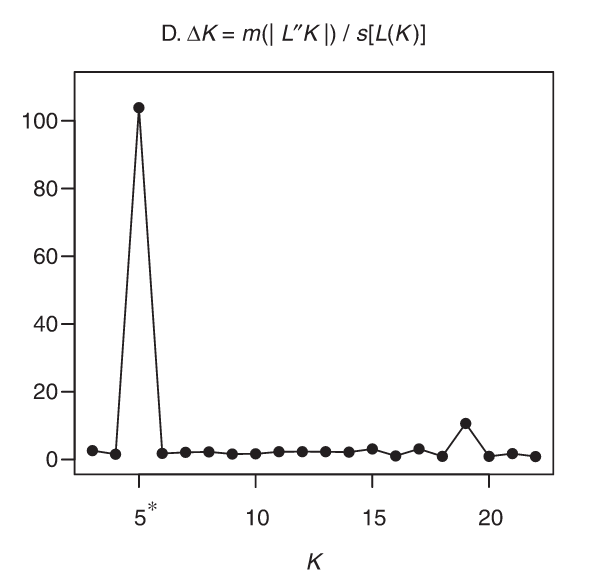
\includegraphics[scale=0.4]{delta_K} 
\end{figure}
The method offers reasonable results, even for hierarchichal clusters (the population structure in the highest hierarchy layer is the expected result), however it was conceived only as an adhoc solution strongly reliant on the results outputed by the STRUCTURE algorithm. Furthermore, there are indications that the method is biased towards lower $K$s if not several exhaustive sampling with the MCMC is completed, which tends to be at least computationally very time comsuming as the dimension of genotype data has rapidly expanded with the introduction of more modern genom sequencing equipment.\\

A more recent approach involves the insight that cluster structure is also resembled in a structured form in the spectrum of the covariance matrix from the respective data. The connection between the spectrum of a matrix and its clustering structure has been subject to research for a fair amount of time. It was first discovered in graph theory \cite{donath1973lower} \cite{fiedler1973algebraic} and later introduced into machine learning \parencite{shi2000normalized, meila2001random, ng2002spectral} for further information see \cite{von2007tutorial}. In general the relevant insight states that: suppose $K$ clusters can be observed in the data matrix $X$ (w.l.o.g. $X$ is a square matrix), then the first $k-1$ eigenvalues $\lambda_1 \geq \lambda_2 \geq \cdots \geq \lambda_{k-1}$ are significantly larger than the remaining eigenvalues, also the corresponding eigenvectors. The number of clusters can thus be inferred by examining the eigenvalues of the data.\\ the In the context of inferring the number of populations by exploiting the appearence of population structure in the eigenvalues was firstly applied by \cite{patterson2006population}. They used insights from random matrix theory, which state that (under various assumptions, like the covariance matrix has properties of a random Wishart matrix) the significant $K-1$ eigenvalues are approximately Tracy-Widom distributed. The Tracy-Widom distribution describes the distribution of the largest eigenvalue for varoius random gaussian matrix ensembles, like the Gaussian orthogonal ensemble ($\beta = 1$) to which the Wishart-matrix belongs. A statistical test is constructed where the eigenvalues are checked with a chosen p-value if there is substantial evidence for the eigenvalue to be Tracy-Widom distributed. \textbf{Performancewise, the method tends to overestimate the number of populations need source!!!.}\\

Further research has been made with random matrix theory (RMT) to concretise the behaviour of the first $k-1$ eigenevalues, including, under certain assumptions, a mathematicaly quantifieable threshhold that destinguishes significantly larger eigenvalues from lower ones. \cite{bryc2013separation}, indicating further that it is only necessary to detect the jump point in the eigenvalues to infer the number of populations. Therefore, instead of relying on ad hoc heuristics or attempting to formulate xpecific mathematical methods with multiple underlying assumptions which in turn have trouble with real data, the use of a machine learning technique that generalises the connection between the number of populations present in genotype data and the correlating structure observed in the eigenvalues.\\

A natural approach for solving problems involving clustering, would be to use well established and commonly used methods, like maximising the likelihood of an expactation maximisation in combination with a model quality estimator such as the Bayesian Information Criterion to counter overfitting. In general bayesian approaches, sucha as maximising the likelihood with regard to a theoretical model of the population structure is always a possible approach, however makes the estimation of the number of populations highly dependable on the a-priori assumptions of the model for what determines mathematically a new population \cite{falush2003inference}. Fitting a hierarchical tree model with bayesian methods has also been attempted \cite{corander2004baps}. Different assumptions from different models could lead to different estimations, which would undermine their comparability. Nevertheless, a maximum-likelihood approach was implemented in the software STRUCTURE \cite{pritchard2000inference} \cite{falush2003inference} and widely applied \cite{rosenberg2002genetic} \cite{harter2004origin} \cite{rosenberg2001empirical}. Furthermore, in some cases, especially for data that involves a high number of populations, a very distinctive maximum is not obtained, for the maximum-likelihood function tends to be smoother as higher values are examined \textbf{more explanation???}. Some approaches add further heuristics, such as also taking the second order rate of change of the likelihood function into consideration \cite{evanno2005detecting}, which however appears more like mending the performance of an approach that was solely conceived as preliminary remedy \cite{pritchard2000inference}.\\
A more recent approach involves the insight that a cluster structure is also resembled in a structured form in the spectrum of the respective data matrix. The connection between the spectrum and a matrix was first discovered in graph theory \cite{donath1973lower} \cite{fiedler1973algebraic} and later introduced into machine learning \cite{shi2000normalized} \cite{meila2001random} \cite{ng2002spectral}, for further information see \cite{von2007tutorial}. In general the relevant insight states that: suppose $K$ clusters can be observed in the data matrix $X$ (w.l.o.g. $X$ is a square matrix), then the first $k-1$ eigenvalues $\lambda_1 \geq \lambda_2 \geq \cdots \geq \lambda_{k-1}$ are significantly larger than the remaining eigenvalues, also the corresponding eigenvectors \textbf{span a subspace that approximates a simplex with the clusters as vertices???}. The number of clusters can thus be inferred by examining the eigenvalues of the data, firstly detected and applied in the context of population genetics by \cite{patterson2006population}. 
\\
\textbf{examples}
\\
Approaches have been made with random matrix theory (RMT) to concretise the behaviour of the first $k-1$ eigenevalues \cite{patterson2006population}, including a mathematical threshhold that destinguishes significantly larger eigenvalues from lower ones \cite {bryc2013separation}. Utilising insights from random matrix theory furtherly remains its beginnings, so far no well performing method based on RMT has been developed. \textbf{cite ???}




\section{Biological Background}

\textbf{ADD MORE !!!}

\subsubsection{Key words}

\begin{itemize}
\item \textbf{Chromosome:} A DNA molecule that encodes genetic information.

\item \textbf{Gene:} A DNA (or RNA) sequence that specifies the structure of a particular functional molecule.

\item \textbf{Locus:} A particular position on the chromosome, like the position of a specific gene.

\item \textbf{Allele:} A variant form of a given gene. Different alleles can lead to distinct phenotypic traits.

\end{itemize}

\section{Modelling}
The subsequently presented model resembles the hierarchical model implemented in STRUCTURE. A first layer, referred to followingly as the F-layer, originates from \cite{falush2003inference} to introduce the possibility of adjusting the correlation of allele frequencies between populations. The F-layer is responsible for determining the allele frequencies of the populations. The second layer, from now on referred to as the admixture layer, stems from \cite{pritchard2000inference} and allows for individuals to have admixed genotypes. Meaning the frequencies of several populations are partially contributing to the pool from which the genotype of an admixed individual is sampled from. The admixture layer samples the genotypes of the individuals, whereby controling the proportions every population contributes to the genotype of an individual.

The genetic information to evaluate individuals is gathered from specific locations in the genom (loci) that can exhibit known genetic variants (alleles). These specific locations are called markers allow for an easier handling of the demensionality and complexity of a genom for certain tasks, such as classefication. To detect properly the magnitude of difference between the genotypes of two individuals from the same species, a sufficient amount of loci that carry genetic variation have to be used. For modelling SNP variations will be used. The biological meaning of the loci generated by the following model for the task of inferring the number of populations is irrelevant, solely necessary is the fact that at each loci different alleles should exist. Each population expresses the alleles at different frequencies, such that, by the law of large numbers, the more loci are simulated the more seperable the populations should be from another and individuals easierly assignable to a population. From a modelling view, it is the different allele frequencies that define a population. \\

\textbf{add snp is biallelic}
Alleles captured from SNP markers are usually biallelic, for the SNP markers locate a mutation in a single nucleotide base pair. That a base pair is effected by several mutations and these mutations assert themselves in the population is, because of the low chances of single nucleotide being affected by a mutation, very unlikely and therefore the possibilities of more than two alleles at an SNP marker is neglected. This allows for a notation simplification of allele frequencies. Let subsequently  $p_{kl}$ determine the probability that an individual from population $k$ has a mutation at locus $l$. Of course the existince of mutant variant is always relative to some reference genome from which over sufficiently long amount of time mutations formed and were able to gather some share in the allele frequencies of a population.\\

The allele frequencies of a population $k$ at a locus $l$ for an allele $a$ will be denoted as $p_k(l_a)$. For simplification purposes each loci in the model can be interpreted as having only two alleles. The model assumes a point in time where \textbf{no different alleles existed??? or alleles where considered the same???} and overtime mutations introduced new alleles that could asser themselves. However the model does not distinguish between the new alleles, only if an individual carries a mutant variant or not (furthermore ploidity is also ignored). The notation therefore also simplifies for the modell to $p_k(l)$ (probability of having a mutant allele at locus l if from population $k$).

\subsection{Further Model assumptions}
The model assumes several properties:
\begin{itemize}
\item Hardy-Weinberg Equilibrium: Relevant to the modelling is that, wiht a Hardy-Weinberg Equilibrium the allele frequencies within a population do not change, the populations are "stationary".

\item Linkage equilibrium: Loci are independent from one another.

\item \textbf{No hierarchical clusters present, like families in a population???}

\item \textbf{further assumptions ???}
\end{itemize}

\subsection{F-Layer}

\textbf{further informations, reader can consult textbooks}
The motivation for introducing correlation between allele frequencies of populations is that poplutions often originate from a common ancestral population, each population roots from the same starting allele frequencies. Reasons for the emergence of new populations are numerous, ranging from geographical divides to social structure impacting the genetic makeup, the common component connecting all is that a  group of individuals excludes themselves sufficiently from mating with the rest of the population and thus practices inbreeding.  Schmetically in population genetics these scenarios of fragmentation are often abstracted as a set of $K$ secluded islands to which some individuals of an ancestral population $A$ migrated and interbreeding on each island occurs.

\begin{figure}
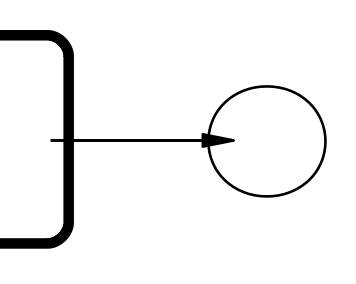
\includegraphics[scale=0.5]{level_1}
\end{figure}

The formation of populations on the islands with distinct allele frequencies is due to a phenomenon called random genetic drift. From a simplified view point, excluding all the biological idiosyncrasies and only looking at the alleles at a single locus, random genetic drift can be seen as an urn model, where the alleles from the locus make up the balls that are drawn from the urn. The proportions of the balls should represent the allele frequencies of the population. The alleles that the offspring receives are sampled from the urn (with replacement). However, since the amount of individuals in the offspring is finite it will most likely not possess exactly the same allele frequencies as as the parents did, causing the allele frequencies of a population to vary until one allele achieves fixation. Fixation occurs when by chance only one specific allele is sampled from the urn, thus eliminating all its competing alleles.\\


The Distinct populations within a species form mainly due to random genetic drift when there is a fragmentation of the general population into subgroups present. Genetic random drift can be interpreted as a stochastic process where the allele frequencies of a gene change randomly over time. The first modelling atempts applied a markov chain \textbf{cite}, where a transition models the change of allele frequencies from one generation to the next. Further refinements have been added over time, such as converting the simplification of discrete populations to the continous case and adding biological idiosyncrasies \textbf{cite}. The random change in the stochastic process stems from the fact that a population has a finite amount of members, whose genetic makeup was "drawn" from a pool with probabilites according to the allele frequencies of the population at the time of the conception of the members, therefore it is likely that the allele frequencies in a population are not passed on exactly. Considering the law of large numbers inversely, the smaller a population is the faster genetic drift will make an impact. The allele frequencies change until one allele is able to assert to fixation, meaning no other variants are substantially left and only the one allele is passed on. \\



All $K$ populations in the model emerged from a single ancestral population $A$. This is founded on the biological background that for  various reasons such as migration, geography, climate, sub popualations form within a single population and as mating between subpopulations decreases or even ceases the populations are effected by distinct random genetic drifts, as a consequence their genetic makeups diverge from another until they can be considered distinct populations. Random mutations and natural selection, if environments are substantially different, in addition support the divergence. \textbf{Nonetheless, the fixation of most genes is mostly due to genetic drift???.} As certain alleles becom more dominant in populations the genetic variation declines and more individuals become homozygous (so less are heterozygous). Using this insight, a divergence statistics that is widely used measures the decrease in heterozygosity between the original population and the newly emerged subpopulation.\\
Let $H_S$ denote the heterozygosity of the original population and $H_T$ the heterozygosity of the subpopulation. Then
\begin{align*}
F_{ST} = \frac{H_S - H_T}{H_S}
\end{align*}
gives a percentage by how much heterozygosity decreased.\\

\textbf{what is the connection to the F-model??? how to get to $\frac{1-F^k}{F^k}$}

This divergence measure, or F-statistic, is used analogously to parametarise the genetic drift from the ancestral population, like following cite{falush2003inference}:
\begin{align}
Dir(p^A_{l_1} \frac{1 - F^k}{F^k}, p^A_{l_2} \frac{1 - F^k}{F^k}, \ldots , p^A_{l_{a_l}} \frac{1 - F^k}{F^k})
\end{align}

Where $p^A_{l_i}$ is the allele frequency from the ancestral population of the allele $i$, from $a_l$ alleles, at locus $l$ and $F^k$ is the drift value of population $k$. At a very low $F^k$ (like $0.05$) the fraction $\frac{1-F^k}{F^k}$ is considerably above $1$, thus the probability mass is mostly concentrated around ancestral allele frequencies. As the value of $F^k$ increases: 
\begin{itemize}
\item for a moderate value (like $0.3$) the probability mass spreads out further, such that more loci will have different allele frequencies and a divergence to the ancestral population is obervable (for a sufficient amount of loci).
\item for a high value (like $0.5$) the probability mass concentrates itself at the vertices of the $k-1$ simplex. This corresponds to a high chance of allele fixation. The fixation will be more likely for the allele that was dominant, mathematically because of the multiplication with $p^A_{l_i}$ in the ancestral population, to begin with. 
\end{itemize}


A population is defined by its allele probabilites, whereby the members of the population are approximately homogenous. The allele probalities are a categorical distributions over the possible alleles at each locus, so how often a genetic variant appears in a population. So at principal, to simulate a new population, its allele probabilities have to be determined. The simulated data the modell produces is supposed to resemble SNP data, where no distinction is made between the different variants of a mutation, but solely if a mutation at ll exists compared to an undetermined hypothetical origin population.

The modell has a hierarchical structure starting with allele probabilities that are derived from an unseen ancestral population. Let $p_{A}(l)$ denote the probability, sampled from a uniform distribution, of an individual from the ancestral population $A$ having a variation at locus $l$. Subsequently, following the genetic drift modelling from (1) by \cite{falush2003inference}, for each population $k$ an F-value $F^{k}$ is chosen to introduce the magnitude of genetic drift from the ancestral population. These are used to derive the mutation probabilities of population $k$ at locus $l$:

\begin{align}
p_{k}(l) = beta(p_{A}(l) \frac{1 - F^k}{F^k}, (1-p_{A}(l)) \frac{1 - F^k}{F^k})
\end{align}

The dirichlet distribution from (1) degenerates to a beta distribtion as effectively only two alleles are considered for each locus. \\

Proceeding, the probability values are joined to a vector $p_k$ and then merged with all other $K$ populations to a matrix $\mathbf{F} = [p_1 p_2 \ldots p_K]^T$ of size $K \times L$, where $L$ is the number of loci, such that each column of $\mathbf{F}$ gives the probabilities of each population for a specific locus $l$. \\

\subsection{Admixture Layer}

Apart from populations drifting from another apart, individuals of populations also migrate and mate with other individuals of other populations. Another modelling layer, according to the admixture model presented in \cite{pritchard2000inference}, introduces the prospect of modelling their admixed offspring, whereby the flexibility, by determining the hyperparameters of a dirichlet distribution, allows to specify the probabilites of how populations partake to what degree in the admixture.

\begin{figure}
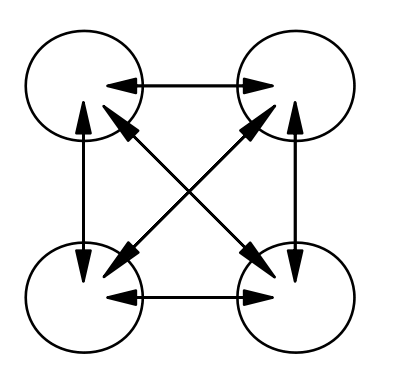
\includegraphics[scale=0.5]{level_2}
\end{figure}

An admixed individual is defined by possessing a mixture of genetic data from various populations. The mixture is a weighting modeled by a categorical distribution according to the influence of each population on the individual. For an individual $i$ the mixture weights $q_i$ are sampled from a dirichlet distribution with $K$ influencing hyperparameters $j_1, j_2, \ldots, j_K$ each corresponding to a population, thus $q_i \sim dir(j_1, j_2, \ldots, j_K)$. A non admixed individual $j$ also receives mixing parameters with the difference that the only non-zero value is a one at position $k$, indicating that the individual belongs to population $k$, so $q_j = [0_1, \ldots, 1_k, \ldots, 0_K]^T$. All $M$ individuals are combined to a mixing matrix $\mathbf{Q} = [q_1,q_2, \ldots q_M]^T$ of dimensions $M \times K$. \\

\subsection{Combining the Layers}

The mixing weights of each individual are subsequently applied over the mutation probabilites of all populations at each locus, which equals to the multiplication of both established matrices $\mathbf{P} = \mathbf{Q}\mathbf{F}$. The resulting matrix $\mathbf{P}$ of dimension $N \times L$ holds the mutation probabilities of each individual for each locus. By using each entry of $\mathbf{P}$ to sample a value from a bernoulli distribution, for either an individual has a mutant allele or not, the simulated SNP genotype data for each individual is obtained. Furthermore, ploidity is neglected, so it is assumed the genetic data is aploidic, since \textbf{ploidity adds nothing unique for the means of inference. citation needed???}, each loci of an individual requires only one sample from the bernoulli distribution.\\

\subsection{Summary}
In summary the generation of a new population setting for which the number of populations $K$ is known proceeds as following:
\begin{enumerate}
\item Sample the ancestral allele frequencies $p_A(l) \sim Uniform(0, 1)$
\item Determine the F-values $F^k$ \textbf{???}
\item  For each of the K populations:
\begin{enumerate}
\item Sample $p^k(l) \sim beta(p^{A}_{l} \frac{1 - F^k}{F^k}, (1-p^{A}_{l}) \frac{1 - F^k}{F^k})$
\item Combine allele probabilities into matrix $\mathbf{F}$
\end{enumerate} 
\item For each individual $i$:
\begin{enumerate}
\item Choose admixture coefficients $q_i \sim Dir(\alpha_1, \ldots, \alpha_k)$
\item Combine admixture coefficients into matrix $\mathbf{Q}$
\end{enumerate}
\item Calculate admixture $\mathbf{P} = \mathbf{Q}\mathbf{F}$
\item Convert each value $p$ of $\mathbf{P}$ by sampling $bernoulli(p)$
\end{enumerate}

\subsection{Looking at Admixture}
The admixture of an individual is determined by the Dirichlet distribution. The dirichlet distribution is parameterised by $K$ hyperparameters $\alpha_1,\alpha_2, \ldots, \alpha_k$. $K$ corresponds to the desired dimension of the output. The probability density function
\begin{align*}
f(x_1, \ldots, x_K, \alpha_1, \ldots, \alpha_K) = \frac{1}{\Gamma(\sum} \cdots
\end{align*}
where $\sum^{K}_{i =1} x_i = 1$ and all $x_1 \geq 0$. So the Dirichlet distribution defines a probability density on the $K-1$-simplex and is therefore a natural choice for sampling admixture coefficients. \\
Of particular interest for the described modell are the hyperparameters, also called concentration parameters, as they control the mode and the variance around it. For values $a_i \geq 1$ the distribution has a single mode, whose coordinates at the maximum $x$ is given by \cite{bishop2006pattern}: 
\begin{align*}
x_i = \frac{\alpha_i - 1}{\sum^K_{k=1} a_k -K} \\
\end{align*}
The mode moves therefore more towards those directions, simplex vertices that have a relatively higher valued corresponding hyperparameter compared to the other hyperparameters. In addition, the variance $\sigma$, given by 
\begin{align*}
\sigma_i = \frac{\alpha_i(\alpha_0 - \alpha_i)}{\alpha_0^2(\alpha_0 + 1)}
\end{align*} 
where $\alpha_0 = \sum^{K}_{i = 1} \alpha_i$, reaveals that higher values of hyperparameters leads to a decrease of the variance, meaning a higher concentration around the mode. \\
These two properties can be exploited to control the probability of sampling certain admixture coefficients. Furthermore, by sampling from the same dirichlet distribution one is able to simulate various population scenarios, such as a detached admixed cluster, which would correspond to a mode with high concentration parameters, or a population that experienced migration, which would coincide with a degenerated dirichlet distribution that only has two nonzero, concentration values for the two involved population, which is in the end a beta distribution.

\subsection{Analysis}
The population centroids given by the population allele frequencies (they are the probabilities used for the bernoulli sampling and thus the mean) construct the vertices of a simplex in which the individuals approximately lie. Outliers are solely due to the natural variance created by sampling at the end from a bernoulli distribution. The probabilities the genetic information from each individual is sampled from, nonetheless always combine to a vector that lies within the simplex, for the probabilities are through the admixture coefficients a linear combination of the population allele frequencies or, in other words, of the simplex vertices. From another perspective, the matrix $\mathbf{F}$ that holds the centroids of the populations as rows, then the matrix maps every vector $s$ from the support of an $L$ dimensional dirichlet distribution accordingly on to the simplex spanned by the centroids (so $\mathbf{F}s$). The matrix $\mathbf{F}$ linearly transforms the $L$-simplex to the desired population simplex.

For further assessment a mean of quantifying the disimilarity between two individuals is necessary. As a measure of genetic distance between two individuals $i$ and $j$ a natural choice is to use a normalised manhatten distance because the possible values of the genetic information of an individual lies on a lattice of values zeros and ones. Or more concrete, let $N$ be the number of loci used as genetic markers, then $\{0,1\}^N \subseteq \mathbb{R}^N$  is the set containing all possible values for the genetic information of an individual. The measure of genetic distance is 

\begin{align*}
D = \frac{1}{N}\sum^{N}_{n = 1} |l^i_n - l^j_n|
\end{align*}

where $l^i_n$ and $l^j_n$ are the values of individual $i$ and $j$ respectively at locus $l_n$. The normalisation keeps the measure invariant to the number of loci used, as recovering more genetic information should not increse the genetic distance per se. The measure ranges from $0$, as two individuals are genetically similar, to $1$, meaning genetic disimilarity.
\\
Suppose two individuals $i$ and $j$ are generated by the described modell, so sampling from a bernoulli distrebution for each loci $l$ with the respective allele frequencies $p_i(l)$ and $p_j(l)$. The expected genetic difference of both individuals then is: 
\begin{align*}
\mathbb{E}[D] &= \frac{1}{N}\sum^{N}_{n = 1} \mathbb{E}[|l^i_n - l^j_n|] \\
&= \frac{1}{N} \sum^{N}_{n = 1} p_i(l)(1-p_j(l)) + p_j(l)(1-p_i(l))
\end{align*}
The result is intuitive. It is the the empirical mean of sampling diffirent allele values. \\
For individuals sampled from the same probabilities the expectation equates to:
\begin{align*}
\frac{2}{N} \sum^{N}_{n = 1} (p(l) - p(l)^2)
\end{align*}
\textbf{the further apart allele frequencies -> not always higher gentic difference. measure bad ?!}
\\
By investigating the variance of two individuals sampled from the same allele frequencies a better impression of the cluster (population) density can be obtained. Also the expected severity of individuals lying outside the simplex can be assessed. \\
But before calculating the variance, for simplicity reasons the expectation of the genetic difference squared is calculated:

\begin{align*}
\mathbb{E}[D^2] &= \frac{1}{N^2} \mathbb{E}[(\sum^{N}_{n = 1} |l^i_n - l^j_n|)^2] \\
&= \frac{1}{N^2} \sum^{N}_{n = 1}\sum^{N}_{m = 1}\mathbb{E}[ |l^i_n - l^j_n||l^i_m - l^j_m|] \\
&= \frac{1}{N^2}( \sum^{N}_{n = 1}\mathbb{E}[|l^i_n - l^j_n|^2] + \sum^{N}_{n = 1}\sum^{N}_{\overset{m = 1}{m \neq n}} \mathbb{E}[|l^i_n - l^j_n||l^i_m - l^j_m|]) \\
&= \frac{1}{N^2}( \sum^{N}_{n = 1}2(p(l_n) - p(l_n)^2) + \sum^{N}_{n = 1}\sum^{N}_{\overset{m = 1}{m \neq n}} 4(p(l_n)-p(l_n)^2)(p(l_m)-p(l_m)^2) \\
\end{align*}

and since
\begin{align*}
\mathbb{E}[D]^2 &= \frac{4}{N^2}( \sum^{N}_{n = 1}\sum^{N}_{m = 1} (p(l_n) - p(l_n)^2)(p(l_m)-p(l_m)^2)\\
\end{align*}
The variance simplifies to
\begin{align*}
Var(D) &= \mathbb{E}[D^2] - \mathbb{E}[D]^2\\
&= \frac{2}{N^2} (\sum^{N}_{n = 1} (p(l_n) - p(l_n)^2) - 2\sum^{N}_{n = 1} (p(l_n) - p(l_n)^2)^2) \\
&= \frac{2}{N^2} (\sum^{N}_{n = 1} p(l_n) - 3p(l_n)^2 + 4p(l_n)^3 - 2p(l_n)^4)
\end{align*}
This reveals that the variance decreases significantly of the order $\mathcal{O}(N^{-2})$ with the number of loci. Therefore, less severe outliers and better observable clusters are to be expected the more loci are simulated.

\subsection{Relationship to LDA}
The presented modell is strongly related to a modell more commonly known under the name latent dirichlet allocation (LDA) \cite{blei2003latent}. LDA uses in the setting of natural language processing (NLP) an ensemble of words that are probabilistically associated with certain topics, in order to determine which topics are exhibited by analysed documents, that preferably possess some associated words. Since not all existing words are associated with topics but only a selection, the selected words can be perceived as reasonable indicators of the topic context, as are the used genetic markers to determine population affiliation. A one hot encoding of wether a word is present in a document or not is the respective equivalent of wether an individual possess a gene variant at a genetic maker or not. The encoding of the selected words or respectively of the genetic markers span the feature space in which the topics/populations lie. The topics/populations then span a simplex in which the documents/individuals are mapped according to the admixture. \\

%\begin{align*}
%\mathbf{Q} = \begin{bmatrix}
%q_1^T \\
%q_2^T  \\
%\vdots  \\
%q_n^T
%\end{bmatrix}
%\end{align*}


\section{Theory}

\subsection{Approximate Bayesian Computation}

At heart of approximate bayesian computation (ABC) lies the inference of a desired parameter value $\theta$ for given data $D$ by relating the conditional probability of that data given the parameter value $P(D | \theta)$ to the symmetric counter part, the conditional probability of the parameter given the data $P(\theta | D)$. This is done by exploiting Bayes' rule:

\begin{align*}
P(\theta | D) = \frac{p(D | \theta) P(\theta)}{P(D)}
\end{align*}

Where $P(D | \theta)$ is often called the likelihood, $P(\theta | D)$ the posterior, $P(\theta)$ the prior and $P(D)$ the evidence which is used in Bayes' rule solely for nomalisation porpuses. \\
For many problems the problem space is intractable or dimensionally too large to compute the likelihood. ABC intends to circumvent these problems.

\subsubsection{Rejection Algorithm}
The rejection algorithm employs a basic approach for finding the posterior distribution of the desired parameter $\theta$ for specific data $D$. Given a known prior distribution of $theta$, the algorithm samples values $\hat{\theta}$ from the prior and then inputs $\hat{\theta}$ into an appropriate model to simulate some data $\hat{D}$. If the simulated data lies with in a margin of error $\epsilon \geq 0$ from data $D$ for a chosen metric $\rho$ , so $\rho(D, \hat{D}) \leq \epsilon$, then the sampled prior value $\hat{\theta}$ is accepted by adding it to the final sample of parameter values for $\theta$. The final sample should approximate the desired posterior. For further infromation and possible refinements such as using linear regression to counter the error at acceptance or using Sequential Monte Carlo - ABC to sample from areas with higher posterior density the reader is referred to \cite{csillery2010approximate}. \\
If the task is for example to compare different models concerning a specific data set, a variant of the rejection algorithm usually poses a reasonable choice. For tasks that only require a good point estimate of $\theta$ that fits well to the data $D$, like the maximum a posteriori (MAP), the rejection algorithm might be too elaborate. Also, the algorithm does not generalise over all possible data sets, meaning it has to be rerun each time for other data, which could be computationally costly. Furthermore, the explicit construction of a model that simulates data introduces assumptions into the computation, as this is a further approximation it is potentially problematic for the decency of the approximation. \textbf{use instead implicit models like GAN???} \\

\subsubsection{In Context of Supervised Learning}
In contrast to the rejection algorithm, supervised learning techniques, such as neural networks or boosting decision trees, address all the problems stated above. A supervised learning method attepmts to find a general connection between any given input data $D$ and its desired output $\theta$ by training a malleable model. The model is instructed to infer the general connection by adapting itself in such a way that it minimises the emperical risk (for some chosen loss function) when solving a finite training set of size $N$, which is a data set with "presolved" values $((D_1,\theta_1),\ldots (D_N,\theta_N))$. From another perspective, a supervised learning algorithm attempts to forge a model in such a way that it perfects the approximation of the \textbf{problem space???} and thus returns good point estimates for $\theta$ given any input data $D$. \textbf{what about the posterior, are the returned values the MAP???}. The prior $P(\theta)$ can be implicitly adjusted by changing the proportions of $\theta$ in the training data.\\
The quality and size of the training set partakes hugely in achieving good results for supervised learning methods. \textbf{By generating synthetic data it is possible to easily construct a plenteous data set, however this again introduces prior assumptions into the learning process and undermines the goal of generalisation. A measure to counteract this problem is to rely on summary statistics that focus on the relevant statistics for the task at hand.??? regularisation through insufficient statistics???}

\subsubsection{Summary Statistics}
Large dimensionality of a data set can undermine the practability of an ABC-method. By summarising the data one attempts to reduce dimensionality, while still sustaining a good approximation of the posterior. So if $S(D)$ is a summary statistics of some data $D$ then the acceptance criterion for the rejection algorithm converts to $\rho(S(D), S(\hat{D})) \leq \epsilon$, whereby $P(\theta|D) \approx P(\theta|S(D))$ holds sufficiently. The use of summary statistics is not confined to the rejection algorithm, rather it is a general tool that allows for a tradeoff between reduction of dimensionality and the goodness of the approximation, since each summarisation usually forfeits some of the principal information. If no information is lost, so $P(\theta | D) = P(\theta| S(D))$ applies, then the summary statistics is called sufficient. \textbf{However, only exponential families have finite sufficient summary statistics, for they are maximum entropy distributions???}. A good informative choice of summary statistics is highly task and data set dependent \cite{nunes2010optimal}. An overview of common heuristics and algorithms for choosing summary statistics can be found in \cite{blum2013comparative}.

To infer the number of populations $K$ expressed in a given dataset $X$ the conditional probability $P(K | X)$ with respect to $K$ is maximised. Since the large dimensionalities of the used datasets pose substantial computational difficulties, the datasets are summarised  in an effective manner, such that the approximation $P(K|X) \approx P(K | sum(X))$ is sufficient for the intended inference. Bayes' theorem then yields

\begin{align*}
P(K | sum(X)) = \frac{P(sum(X) | K) P(K)}{P(sum(X))}
\end{align*}

The calculation of the likelihood $P(sum(X) | K)$ however is intractable because \textbf{???}
To circumvent this problem the likelihood is implicitly calculated by employing a supervised learning method to estimate the posterior, such as a neural network or boosting decision trees. These methods are trained by trying to link summary statistics of datasets to the corresponding values for the number of populations. The prior $P(K)$ 
can be implicitly adjusted by changing the proportions of $K$ in the training data. Gradient boosting with decision trees is chosen in this case, for it has demonstrated good results for various classification problems citation needed. \textbf{??? Furthermore, some inuitive reasoning exists, as explained later on, for the use of decision trees in this particular case.}

\subsection{Choosing the Summary Statistics}

The choice of adequate summary statistics is essential to obtain significant results. Large dimensional data often times demands it to be summarised, so the intended methods a reasonably applicable. In doing so, the manner summary is of great importance because each summarisation usually forfeits some of the principal information. So one is confronted with the problem of how to effectively manage the trade off between the practicability the method and the loss of information that could endager desired results.\\
The entropy of a distribution measures the existing uncertainty about which event appears if one samples from the distribution. Mathematically it is defined for a given continous probability mass function $P(X)$ as
\begin{align*}
h(x) = - \int_{supp(P)}P(x)\log(P(x))dx
\end{align*}
The principal of maximum entropy states that given some prior information about the underlying probability distribution, such as already drawn samples or a constraining property, the maximum entropy distribution that incorporates the prior information is the best distribution to respect the remaining uncertainty \cite{jaynes1957information}. In other words, the maximum entropy distribution is the best distribution to fit the already obtained information if no further assumptions are to be added. \\
For a given mean $\mu$ and covariance $\Sigma$ the multivariate continuous distribution that maximises the entropy is the multivariate Gaussian, for a proof the reader is referred to \cite{cover2012elements}.
The entropy of the multivariate Gaussian is derived as following:

\begin{align*}
h(x) & = - \int_{-\infty}^{\infty} N(x|\mu, \Sigma)\ln(N(x|\mu, \Sigma))dx \\
& = E[\ln(N(x|\mu, \Sigma)] \\
& = E[\ln(det(2\pi\Sigma)^{-\frac{1}{2}}e^{-\frac{1}{2}(x-\mu)^T\Sigma^{-1}(x-\mu)})] \\
& = \frac{1}{2}\ln(det(2\pi\Sigma)) + \frac{1}{2} E[(x-\mu)^T \Sigma^{-1}(x-\mu)]\\
& = \frac{1}{2} \ln(det(2\pi\Sigma)) + \frac{1}{2} E[trace(\Sigma^{-1}(x-\mu)^T (x-\mu))]\\
& = \frac{1}{2} \ln(det(2\pi\Sigma)) + \frac{1}{2} E[trace(I)]\\
& = \frac{1}{2} \ln(det(2\pi e \Sigma))
\end{align*}

The only non-constant factor influencing the entropy of a multivariate gaussian is the determinant of the respective covaraince matrix.
Since any real symmetric matrix is diagonalisable, $det(\Sigma)$ breaks down to $det(\Sigma) = det(\mathbf{Q}^{-1}) \cdot det(\mathbf{\Lambda})\cdot det(\mathbf{Q}) = \prod_{i = 1} \lambda_{i}$, thus revealing that actually the eigenvalues of the covariance matrix are responsible for the magnitude of the entropy. In conclusion, by summarising the data by its covariance matrix, one implicitly approximates the data as being guassian and secondly it suffices for the summary to only take the eigenvalues into consideration.

\textbf{Assume Data is linearly correlated??? connection to PCA???}

\subsubsection{PCA}

\textbf{add introduction???}
Principle component analysis is a statistical method that performs a basis transformation on a given data set, such that no linear correlations are anymore present in the data. Since the direction of a linear correlation corresponds to the direction of the highest variance in a concerning subspace, a new axis musst be aligned according that particular direction. \textbf{citation needed ???} This construction of the axes is done by requiering in an iterative manner each new axis to align with the direction that captures the most variance in the data, which however has not been captured by already established axes. \\
The differences between data points makes them destingiushable, but also determines the magnitude of the observed variance. Decreasing the variance in a data set by projecting it into a subspace, thus endagers destinguishability (in certain features or even in total), which is information. The amount of sustained variance after projecting the data into a subspace can therefore act as an indicator for how much information was retained. So by always maximizing the captured variance of a newly added axis to the transformation, which is a subspace of the principal data set, the highest possible amount of information is retained for a projection into a subspace with a particular rank $K$ (under the assumption that variance corresponds to information). The subspace is spanned by the $K$ largest Eigenvectors \textbf{singular values ???} of the empirical covariance matrix, as is subsequently shown. \\
Let $S = \frac{1}{N}XX^T - \overline{X} \overline{X}^T$ denote the emperical covariance matrix of the data matrix $X$. Then the expression $u^TSu$ is the emprical variance of $u^TX$, which is the data $X$ projected on to the vector $u$.

\begin{align*}
u^T S u & = \frac{1}{N} u^T X X^T u - u^T \overline{X} \overline{X}^T u \\
& = \frac{1}{N} u^T X (u^T X)^T  -  \overline{u^TX} (\overline{u^TX})^T  \\
& = \frac{1}{N} (u^T X)^2 - (\overline{u^TX})^2
\end{align*}

The empirical variance is maximised with the restriction $\parallel x \parallel = 1$ because $u$ is supposed to be part of a new standard basis. \textbf{mention orthogonality ???}. By using a lagrange multiplier to add this restriction, the equation $\max\limits_{u} u^T \Sigma u - \lambda(u^T u - 1)$ is obtained.

\begin{align*}
 \frac{d}{du} (u^T \Sigma u - \lambda(u^T u - 1)) & = 0 \\
 \Sigma u - \lambda u & = 0 \\
 \Sigma u & = \lambda u 
\end{align*}

The solution coincides with the definition of the Eigenvectors, where $\lambda$ is the eigenvalue of $u$. Since $u$ should be maximised, the overall solution is the eigenvector belonging to the largest eigenvalue.

\textbf{Add explanation of SVD??}

\subsubsection{In context to clustering}
Cluster analysis intends to group similar data points together. \textbf{what are the clustering assumptions??? distribution? group criteria? bounderies?}
Data that exhibits reasonable clustering possess a considerably unique structure. This structure also reveals itself to some degree in the orientation of the eigenvectors and the magnitude of the corresponding eigenvalues, such that they can be utilised to infer certain properties of the data, like the number of clusters as is the current intention. \\
Intuitively, for inferring the number of clusters, it is assumable \textbf{cluster assumptions} in a reasonable setting, including for example that each cluster has a at least a minimal amount of members, that the in-between variance between two distinct clusters is significantly greater than the variance whith-in a particular cluster. The in-between variance constitutes itself through the variance of the with-in variance of both concerning clusters and the distance between the clusters (under the assumption that outliers are possible, so cluster membership is not compulsive). While the with-in variance of a cluster is solely confined to the space assigned to that cluster, which concludes to a significantly smaller variance, espacially considering that the distance of each data point to the mean has a squared impact on the variance (definition of variance). For these reasons a new principal component will orient itself in such a way, that it effectively captures the remaining in-between variance of the clusters. \\
For $K$ many different population clusters $K-1$ significant PCs are obtained, thus allowing an inference of the number of populations. Considering only two clusters, a single significant PC would be observed that is oriented along a line connecting the two centroids of each cluster, as this would maximise the distance of the clusters after a projection on the PC and therefore maximise the variance after projection. In a general setting with $K$ clusters, the PCs would arrange themselves as linear combinations of the in-between variances, as the overall variance is maximised so all in-betwenn variances are taken into account. Since every cluster participates in $K-1$ in-between variances and capturing these in-between variances corresponds to determining the \textbf{exact??? (the centroids???} relative positions of the other cluster, a linear combination of exactly $K-1$ vectors are needed to locate the relative positions of the other clusters \textbf{proof necessary??? less: would mean a cluster is admixed, admixture = linear combination of existing clusters $\rightarrow$ contradiction | more: some in-between variance was not captured - contradiction to maximising variance, sufficient???}. \textbf{The centroids lie in the span of the first $K-1$ PCs ???}

The past mentions of population clusters solely referred to clusters that are not admixed. The introduction of admixed population clusters, however does not alter the previously established theory under certain assumptions. Admixed clusters are several individuals with similar admixed genotypes and are sampled from allele probability values that are subject to a mixture weighting of the allele probability values of the non-admixed populations according to their involvement in the admixture as done in the modell (2). This is simply a linear combination, restricted to the coefficients being proportions (summing to one), of the centroids of the other populations, meaning an admixed individual and therefore the centroid of an admixed cluster lie also in the span of the $K-1$ first PCs spanning the non-admixed populations. In general, the centroids of the non-admixed populations constitute the corners of a simplex, that determines if a population cluster is admixed, thus the influence of admixed individuals concerning the maximisation of the variance is neglegible. \textbf{further explanation needed???}.

\subsection{Examples}
A synthetic problem instance generated by the modell, could look like shown in Figure 1, where three populations that span the simplex are observable. The populations have fairly distinct F-values (meaning they drifted away from the ancestral poulation at quite different magnitudes), therefore the clusters are well seperable from one another. Within the simplex is a cluster of several admixed individuals located. They were all sampled from the same dirichlet distribution $Dir(8, 8, 8)$, with uniform hyperparameters, so they are concentrated around a central mode and all populations participate on average the same amount to the admixture. \\
Just by looking at the corresponding biggest eigenvalues, it is fairly easy, with the use of the previously insights, to infer the number of populations. The first two eigenvalues are significantly larger than the rest, thus the number of populations should be three. 

\begin{figure}[h!]
\caption{Projection of three populations and one admixed on to the firs two PCs and corresponding eigenvalues}
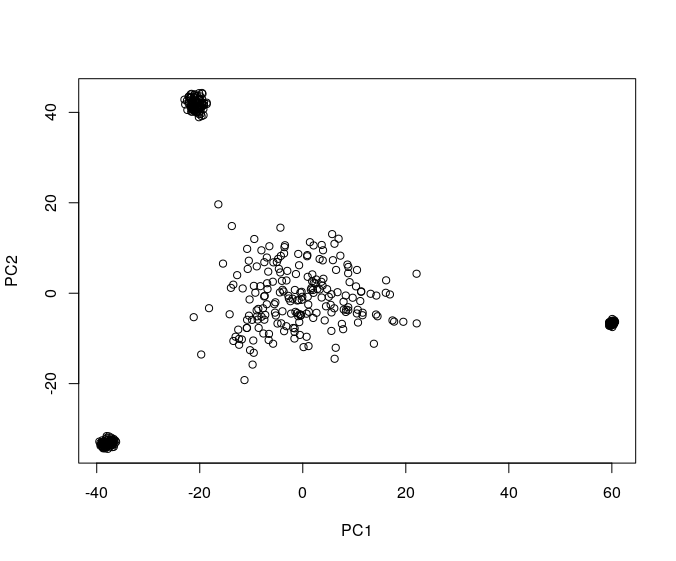
\includegraphics[scale=0.41]{Rplot_projection}
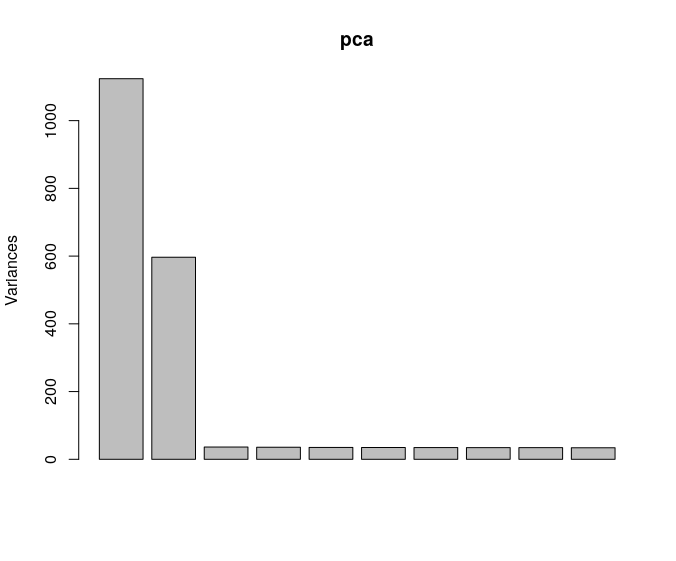
\includegraphics[scale=0.41]{Rplot_eigenvalues}
\\Three populations with F-values  of $0.1, 0.5, 0.9$ and $100$ individuals each were sampled. The admixed population derived the proportional weightings for its allele probabilites by sampling for each allele from a $Dir(8, 8, 8)$ distribution. $200$ individuals were sampled for the admixed. For this simulation $10000$ loci were simulated.
\centering
\end{figure}

Figure 2 shows a similar scenario as Figure 1, whereby the only difference consists of a different admixture of the admixed individuals. In this example admixed individuals are sampled from three different dirichlet distributions. In turn one of the hyperparameters is set to zero, thus always on population does not partake in the admixture of an individual. As a consequence the individuals are spread along the edges of the simplex, also because the non-zero hyperparametes model a lower concentration than in Figure 1. \\
Again the eigenvalues feature two significant large eigenvalues, making the inference of the number of populations using solely the eigenvalues once again a simple task. The natural variance of the descretisation of the allele values through the bernoulli distribution, which would allow individuals to lie outside the simplex, only has a neglectable marginal effect on the eigenvalues.

\begin{figure}[h!]
\caption{Projection of three populations and one admixed on to the firs two PCs}
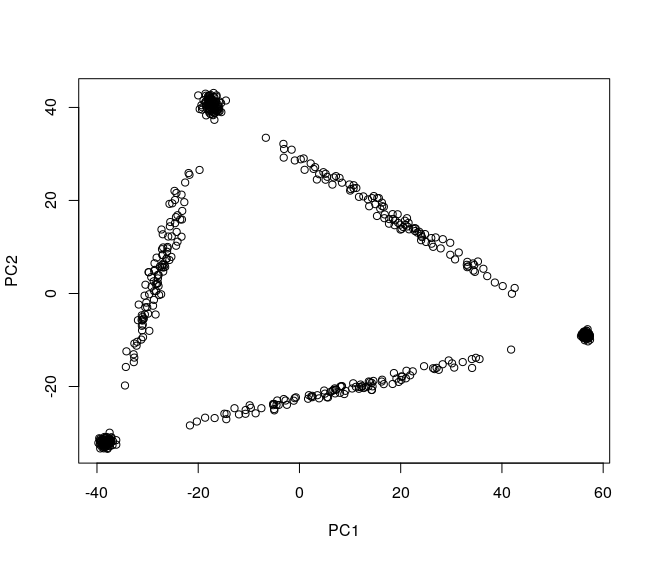
\includegraphics[scale=0.5]{Rplot_admixed_simplex}
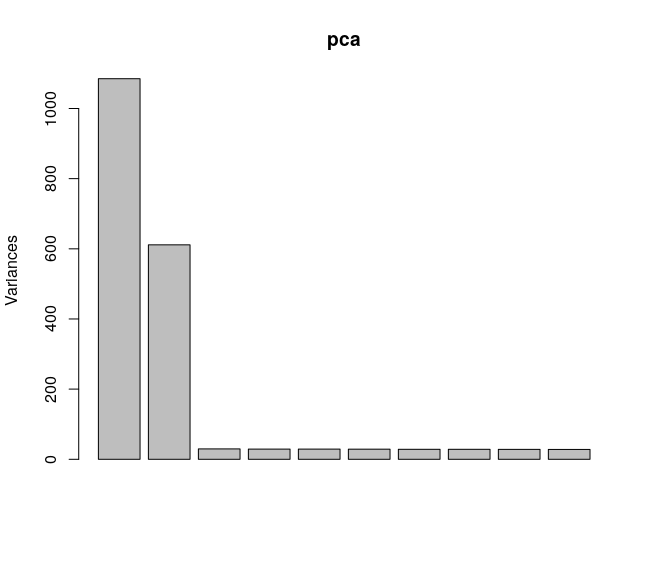
\includegraphics[scale=0.5]{Rplot_eigenvalues_simplex}
Three populations with F-values  of $0.1, 0.5, 0.9$ and with $100$ individuals each were sampled. Between each pair of population clusters lies an admixed population sampled from a dirichlet with $5$s and a $0$ for not involved populations, which corresponds to a $beta(5, 5)$. Each admixed cluster holds $200$ individuals. The simulation used again $10000$ loci.

\centering
\end{figure}


\subsubsection{Difficulties}
The past examples only demonstrate fairly simple problem instances, for which even a human recognition capabilities suffice. It is also possible to construct more difficult problem instances. Figure 3 is an example of such. The ploy is to simulate a setting where most of the variance is already captured by less than $k-1$, hence making it  more difficult to recognise the cut-off for significant and insignificant eigenvalues. In figure 3 there are two populations that have similar allele frequencies (F-values 0.05 and 0.1) and one population that has been subject to strong genetic drift and therefore is genetically completely distinct (F-value 0.99). Furthermore, most individuals are distributed over one of the two close populations and the one very far apart. This introduces high a high incentive for the eigenvalues to try to capture the variance of the individuals of the two populations, since a bigger distance accounts for higher variance. Inversesly, because the population that holds a fewer amount of individuals is not very far away from the positioning of the first eigenvector, such that the second eigenvector, which has to orient itself perpendicular to the first, does not capture very much variance. Also the low amount of individuals in the smaller population makes the orientation of the second eigenvector susceptible to the variance of the other populations or to any outliers. An admixed population also resides between the two greater populations, giving the first eigenvalue even more weight. \\

The graph with the biggest eigenvalues reveals the described dilemma. The first eigenvector accounts for almost all of the variance between the populations, rendering the other significant eigenvalue almost insubstantial and undiscernible from the other insignificant eigenvalues. In different scenarios the distance between the populations and the distribution of the individuals over the populations could be even more disadvantageous (although the question could more be of the nature to decide what is considerable to be a population, \textbf{this is part of the discussion???}). In addition, the situation becomes even more difficult if even more populations are simulated with "extreme" F-values.

\begin{figure}[h!]
\caption{Example of a difficult case}
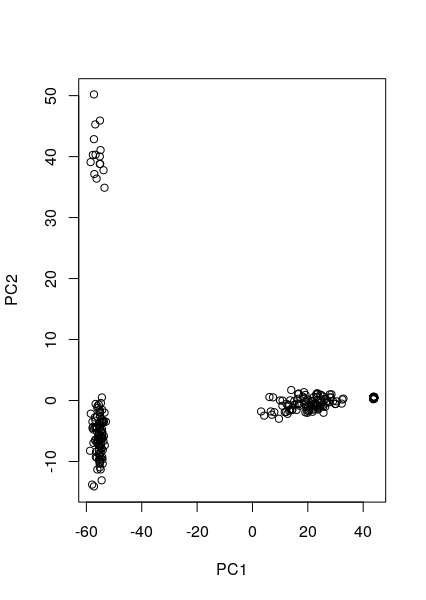
\includegraphics[scale=0.6]{Rplot_hard_example}
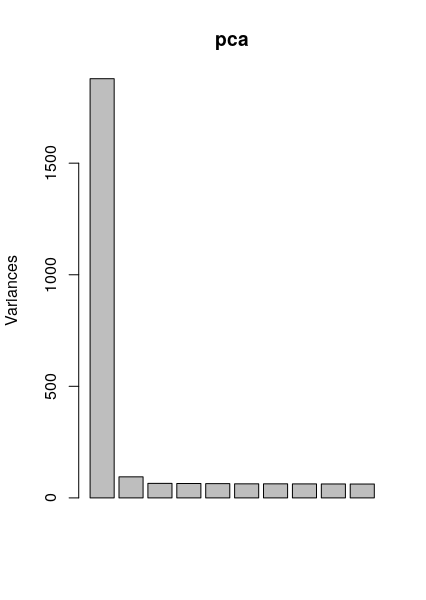
\includegraphics[scale=0.6]{hard_example_eigenvalues}
\\Three populations with F-values  of $0.05, 0.01, 0.99$. The first population with the smallest F-value has $15$ members, while the others have a $100$ each. The mixture proportions of the admixed population were sampled from a $Dir(0, 10, 30)$. $10000$ loci were simulated.

\centering
\end{figure}


\newpage

\subsection{RMT}

Let $\mathbf{A} = \frac{1}{n}\mathbf{X}\mathbf{X}^{T}$ be the empirical covariance matrix of $\mathbf{X}$ with $\mathbf{X}$ being an $m \times n$ matrix. $\lambda_{1},\lambda_{2}, \dots, \lambda_{m}$ are the corresponding eigenvalues of $\mathbf{A}$. The empirical spectral distribution (\textbf{ESD}) for  $\mathbf{M}$ is then given by:

\begin{align*}
F^{M}(x) = \frac{1}{m} \mid \{\lambda_{i} \leq x \mid i \leq m\} \mid
\end{align*}

Whereby $\mid \cdot \mid$ denotes the size of a set.
\\
\\
By assuming a theoretical setting in which $m, n \rightarrow \infty$ while $y = \frac{m}{n} \rightarrow (0, \infty)$ the Marchenko-Pastur Law extends the ESD to the continuous case.

Under the assumption that the entries of $\mathbf{X}$ are random variables iid distributed with mean $0$, it states that the probability density of the eigenvalues is given by:

\begin{align*}
p^{M}(x) = \frac{1}{2\pi xy \sigma^{2}}  \sqrt[]{(\rho_{+} - x)(x - \rho_{-})}
\end{align*}

where $\rho_{\pm} = \sigma^{2}(1 \pm \sqrt[]{y})^{2}$ and $\sigma^2$ is the variance of the random variables.
\\
\textbf{Insert Plot of distribution}
\\

\newpage

\section{Boosting Decision Trees}
Subsequently a concise overview of gradient boosting and decision trees is presented. For further details and idiosyncrasies of the methods the reader should consult more elaborate literature, like \cite{trevor2009elements}.
\subsection{Gradient Boosting}
Gradient boosting is a supervised learning method for classification and regression, that iteratively adds basis learners to a linear combination to reduce an arbitrary differentiable loss function.\\

Let $\chi$ denote the input space. The task then is to approximate the function $f^*(x)$ that maps an arbitrary input $x \in \chi$ to the desired output $y \in \mathbb{R}$. An ensemble of $M$ different basis learners $g_1,g_2,\ldots,g_M: \chi \rightarrow \mathbb{R}$ can be used to generalise over a training set $((x_1, y_1),(x_2,y_2),\ldots,(x_N, y_N))$ of $N$ training pairs in a linear fashion as following:
\begin{align*}
f(x) = \sum_{m=1}^{M}\phi_m g_m(x)
\end{align*}
where $\phi_i \in \mathbb{R}$ are the weights for each basis learner. Linear models for a set of given basis learners can be fitted via konventionell methods such as least squares, lasso, ridge \cite{bishop2006pattern}. $f(x)$ can be used as an approximation for various tasks like regression, classification (by for example using a threshhold), \\

The model is limited by the explicit choice of the basis learners. Instead an algorithm that finds the best base learners from a hypothesis space $\mathcal{H}$ would increase the adaptive potential of the model. Thus, for a given differentiable loss function $l(x, f(x))$, an algorithm should find the best $M$ base learners $h_1, h_2, \ldots, h_m \in \mathcal{H}: \chi \rightarrow \mathbb{R}$ and corresponding weights such that the empirical risk is minimised:

\begin{align}
\argmin_{\phi_i, h_i}\frac{1}{N}\sum_{i = 1}^{N} l(y_i, \sum_{m=1}^{M}\phi_m h_m(x_i))
\end{align}

Solving this task is an optimisation problem usually beyond practicability. A common optimisation technique is too update the parameters through the use of gradient descent. Several problems arise in the case of differentiating over the hypothesis space:

\begin{itemize}
\item Firstly, the hypothesis space would need to be parameterised with finite dimensions. In the face of a countless manifold of possible base learners a rather daunting task. One is far better off by confining the possibilities of base learners, by choosing a subset $H \subset \mathcal{H}$ like decision trees or neural networks.

\item Many modelling frameworks such as neural networks (e.g. number of hidden layers) and decision trees (e.g. tree depth) have to be parametrised at least partly discretely. Of course all discrete model features could be fixed to a constant, but that would greatly degrade the modeling capabilities.

\item Lastly, some base learners do not model a differentiable functions. For e.g. decision trees model functions that possess jump discontinuouties.
\end{itemize}

Gradient boosting algorithms, firstly developed and described by \cite{freund1997decision, friedman2001greedy, friedman2002stochastic}, circumvent the necessity of differentiability by growing the ensemble of base learners iteratively that minimises the empirical risk with respect to so called pseudo residuals.\\

The backbone of an gradient boosting algorithm is constituted by forward stagewise additive modeling, which works as following:
Let $H \subset \mathcal{H}$ be the chosen set of possible base learners.
\begin{enumerate}
\item Initialise with constant like $f_0(x) = 0$
\item For each stage $m \in 1,\ldots,M$:
\begin{enumerate}
\item solve \begin{align*}
\argmin_{\phi_i, h_i}\frac{1}{N}\sum_{i = 1}^{N} l(y_i,f_{m-1}(x_i) + \phi_m h_m(x_i))
\end{align*}
\item Set $f_m(x) = f_{m-1}(x) + \phi_m h_m(x)$
\end{enumerate}
\end{enumerate}

The optimisation step, although the amount of parameters is reduced compared to (3), only possess closed viable solving techniques for a limited amount of loss functions, like L2-loss or exponential loss. More information is provided in \cite{friedman2000additive}. To expand the optimisation step to any arbitrary differentiable loss function, the numerical optimisation via gradient boosting is used. \\

The optimisation procedure fixates at stage $m$ the current estimates made by $f_{m-1}(x)$ of the training data in a vector $\mathbf{f}_m = [f_{m-1}(x_1), f_{m-1}(x_2), \ldots f_{m-1}(x_N)]^T$. \\

The loss function then can be reformulated as:
\begin{align*}
L(\mathbf{f}) = \sum_{i = 1}^{N}l(y_i, \mathbf{f}_i)
\end{align*}

Then the gradient of the loss function is calculated w.r.t $\mathbf{f}$.

\begin{align*}
\hat{h}_m &= \nabla_{\mathbf{f}_m}L(\mathbf{f}_m) \\
&=[\partial_{\mathbf{f}_1} l(y_1, \mathbf{f}_1),\ldots, \partial_{\mathbf{f}_N} l(y_N, \mathbf{f}_N)]^T
\end{align*}

Like in conventional gradient descent algorithms the model is adjusted in a manner that the empirical risk is minimsed along the direction of steepest descent. The direction of steepest descent corresponds to the negative of the gradient, which is $- \hat{h}_m$. Base learners that output differentiable function approximations can express the gradient via chainrule through the adjustable parameters of the model itself (like the weights in a neural network) and hence these are reciprocally changed to minimise the loss. Other base learners on the other hand have to resort to a different strategy.\\
The embedding in the forward additive model allows for the negative gradient $-\hat{h}_m$ to be approximated directly by a base learner. The objectiv of the new base learner $h_m(x)$ consequently concludes therein to approximate
\begin{align*}
h_m(x) \approx -\hat{h}_m
\end{align*}
as well as possible. A possible approach would be to train a base learner on the training data, but where the labels are exchanged by $-\hat{h}_m$.\\
Intuitively, a base learner $h_m(x)$ should be considered as an approximate step in the direction of steepest descent of the emirical risk. Following this setup, the weight $\phi_m > 0$ can be considered as the corresponding step size to be adjusted to ones taste. As a conclusion the iterative construction of the final linear model with gradient boosting
\begin{align*}
f(x) = \sum_{m=1}^{M}f_{m-1}(x) + \phi_m h_m(x)
\end{align*}
is a sequence of gradient descent steps towards a minimum of the empirical risk. 

\subsection{Decision Trees}

Typical decision trees are a supervised learning method that solve a regression or classification problem by segmenting the feature space in to distinct regions, whereby all data points lying in the same region are assigned the same value by the tree. \\

Let ${(x_1,y_1),(x_2, y_2), \ldots, (x_N, y_N)}$ be the training data. The input dimension of a point $x_i$ is $D$.\\

Suppose a tree $T$ partitions the featurespace $X_1, X_2, \ldots, X_D$ into $M$ regions $R_1, R_2, \ldots, R_M$. The response function  outputed by $T$ is given by:
\begin{align*}
f_T(x) = \sum_{m = 1}^{M} c_m I(x \in R_m)
\end{align*}
where $I$ is an indicator function signaling if the input $x$ is part of a particular region. $c_m$ is the response for a region $R_m$. The optimal value of $c_m$ depends on a chosen loss function that should be minimsed w.r.t $c_m$ over all the training points assigned to region $R_m$. As an example, for square loss in a regression setting this would accord to the empirical average of the label values from the training points lying in the region $R_m$. \\

A far more challenging optimisation task is finding the optimal tree that partitions the feature space into $M$ regions, for a given loss function $l$.

\begin{align*}
\argmin_{R_m, c_m} \sum_{i =1}^{N} l(y_i, \sum_{m = 1}^{M} c_m I(x_i \in R_m))
\end{align*}

The possibilities of partitioning feature space grows exponentially with the number of features, rendering the encounter of an optimal tree in most cases computationally infeasable. \\

As an alternative, a greedy approximation approach can be used (CART add citation). The greedy algorithm chooses the best dimension $X_d$ and splitting point $s$ that minimises the loss for the two new regions that arise (w.l.o.g. only binary trees will be considered). The two new regions are defined as:
\begin{align*}
R_1(d, s) = \{X | X_d \leq s\} \qquad R_2(d, s) = \{X | X_d > s \}
\end{align*}

The feature space is divided by a plane that is orthogonal to the axis corresponding to feature $X_j$. The plane cuts the value of $s$ on that axis.\\
The optimisation objective thus reduces to the choice of positioning  the best partitioning plane orthogonal to an axis:
\begin{align*}
\argmin_{s, d}[\argmin_{c_1} \sum_{x_i \in R_1(d,s)} l(y_i, x_i) + \argmin_{c_2} \sum_{x_j \in R_2(d,s)} l(y_j, x_j)]
\end{align*}

The optimisation step yields, for a naive implementation that checks for every dimension the splitting value of a plane between every two neighbouring data points, a worstcase runningtime of $\mathcal{O}(D \cdot N log(N))$ ($Nlog(N)$ for sorting feature values), which is computationally much more feasable. However between two neighbouring data points $x_1$ and $x_2$ there are infinitely many positions to place the splitting plane that evaluate to the same empirical risk. As a convention the splitting value $s$ that lies in the middle of $x_1$ and $x_2$, when they are projected on the axis $X_d$, is chosen by convention. The reasoning is that no further assumptions are to be added through the positioning of the plane and since the splitting of the feature space can be viewed as a bernoulli experiment (data point either lies left or right of plane) the bernoulli distribution with expected value of $0.5$ is the maximum entropy bernoulli. \\

After finding the best split, the procedure is repeated on the newly constructed regions until the desired depth of the tree is reached. Regression and classification trees differ from one another only through the selection of a different loss function. For regression standard loss functions like square loss would be reasonable choices. Classification trees have revealed better results for loss function that reward node purity, so to which degree does a node hold data points of a single class. Such loss functions are for example the gini index or cross entropy loss for classification. From an information theory perspective, node purity leads to a greater reduction in entropy. \\

Growing a too big tree $T_0$ is susceptible to overfitting. A regularisation technique that aids in the construction of a well generalising tree is cost-complexity pruning. The goal of pruning is to find a sub-tree $T \subseteq T_0$, by conflating all hierarchically lower nodes that lead off an internal node into that internal nodes, that minimises:
\begin{align*}
C_\alpha(T) = \sum_{i = 1}^{N} l(y_i, f_T(x_i)) + \alpha |T|
\end{align*}
where $f_T(x)$ is the estimate of Tree $T$ for input $x$ and $|T|$ denotes the number of terminal nodes of $T$. The tuning parameter $\alpha \geq 0$ punishes larger more complex trees according to its value. It resembles the regularisation term of ridge regression. \\
The optimal sub-tree corresponding to a particular tuning parameter $T_{\alpha}$ can be found using weakest link pruning. Weakest link pruning conflates those terminal nodes into an internal node to which the terminal nodes are all adjacent, such that the empirical risk increases minimally. Continuing with this procedure until only the root stub remains gives a sequence of subtrees $T_1, T_2, \ldots, T_n$ in which with a probability of $1$ the optimal subtree $T_{\alpha}$ can be found \cite{breiman1984classification}. Cross validation can be used to find the optimal value for $\alpha$.\\

Decision trees exhibit high variance, meaning that completely different splits occur and thus the output prediction rules change cosiderably when there are minor changes added to the training data. The reason resides inherently with how the splits are chosen in a greedy fashion. For example, two promising features could reduce the loss almost equally much, but just the best of both is considered for the next split. Adjusting the training data slightly by for example adding new data points could possibly change the value of the loss function enough to choose the other feature for a split the hierarchical nature consequently propagates the difference further down the tree. This behaviour reveals that the confinement to the greedy perspective when constructing a tree to some degree neglects the goal of generalisation in return for tractability.\\ %, even when regularisation is applied, decision trees inherently possess the manner to overfit. Instead of approximating a prediction function by iteratively adjusting all the model parameters together, like via gradient descent, the confinement to picking a single feature for splitting disregards 

Remedies that address model stability involve the introduction of bias. The bias-variance tradeoff possess an eminent role in machine learning as its a principle that is prominent for many models. In summary, it describes the forfeit of expected accuracy in return for decreasing the variance of an estimated parameter when the training sample is being varied. Creating an ensemble of decision trees is a widely used and fruitful approach. Ensemble approaches for decision trees include bagging, random forests and as well gradient boosting. Several further refinements improve the quality of an ensemble tree models, including randomly masking different features and training data entries for each tree, as this generates differing trees that place their splits differently and therefore deliver more uncorrelated predictions.

%Furthermore, the greedy algorithm is greatly affected by the horizon effect. Meaning it does not recognise if a split with a lower loss reduction would lead to a split that greatly reduces the loss later on. \\
\section{Results}

\section{Discussion}

\printbibliography

\end{document}